\documentclass[tikz,border=8pt]{standalone}
\usetikzlibrary{calc}


\newcommand{\eradius}{3pt}
\newcommand{\blineouterradius}{7pt}
\newcommand{\blineinnerradius}{1pt}

\newcommand{\bline}[1]{%
    \draw[semithick,blue!80] (#1) circle (\blineouterradius);
    \fill[blue!80] (#1) circle (\blineinnerradius);
}

\newcommand{\radiationcone}{%
    (e) -- (10, 5.5) to [out=14.03624, in=90] (13.5, 4) to [out=-90,
    in=-14.03624] (10, 2.5) -- (e);
}


\begin{document}

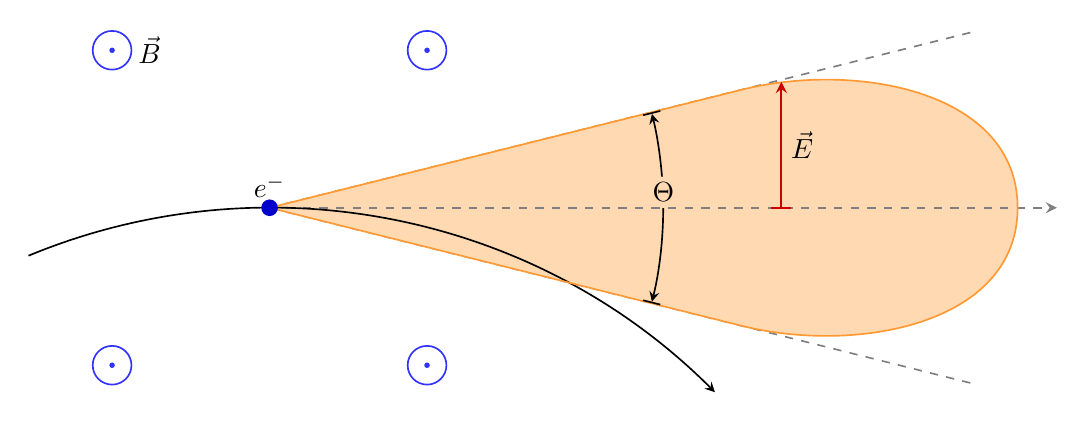
\begin{tikzpicture}[>=stealth]

% gyration center at (4, -4), radius 8

% electron coordinates
\coordinate (e) at (4, 4);

% bline coordinates
\coordinate (B1) at (2, 2);
\coordinate (B2) at (2, 6);
\coordinate (B3) at (6, 6);
\coordinate (B4) at (6, 2);

% dashed radiation cone border
\draw [semithick,dashed,gray] (e) -- (13, 6.25);
\draw [semithick,dashed,gray] (e) -- (13, 1.75);
% radiation cone filling
\fill [orange!30] \radiationcone;
% radiation direction
\draw [dashed,thick,gray,->] (e) -- (14, 4);
% electron trajectory
\draw [semithick,->] (0.93853,3.39104) arc (112.5:45:8);
% radiation cone outline
\draw [semithick,orange!80] \radiationcone;

% draw electron and blines
\fill [blue!80!black] (e) circle (\eradius);
\foreach \bcoord in {B1, B2, B3, B4}
    \bline{\bcoord};

% opening angle of cone
% \draw [semithick,->|] (10.61863,6.27898) arc (19:13.97:7);
% \draw [semithick,->|] (10.61863,1.72102) arc (-19:-13.97:7);
\draw [semithick,|<-] (8.85071,5.21268) arc (14:4.5:5);
\draw [semithick,|<-] (8.85071,2.78732) arc (-14:0:5);
% Efield oscillation
% \draw [thick,red!80!black,|->] (10,3.985) -- (10,5.5);
\draw [thick,red!80!black,|->] (10.5,3.985) -- (10.5,5.6);

% labels
\node [right=6] at (B2) {$\vec{B}$};
\node [above] at (e) {$e^-$};
\node [right] at (10.5, 4.8) {$\vec{E}$};
% \node [right] at (10.6, 6.2) {$\Theta$};
\node  at (9, 4.2) {$\Theta$};

\end{tikzpicture}

\end{document}
